Before commencing any empirical work, it is essential to thoroughly review the existing literature, and the relevant articles that are found can be summarized in the literature review section. This will not only help to put the proposed research in a relevant context, but also may highlight potential problem areas, and will ensure up-to-date techniques are used and that the project is not a direct (even unintentional) copy of an already existing work. The literature review should follow the style of an extended literature reviews in a scholarly journal, and should always be CRITICAL by nature. It should comment on the relevance, value, advantages and shortcomings of the cited articles. Finally you PLACE your research into the body of literature.


\chapter{Literature Review}

\textbf{1. What is IV}
\begin{itemize}
    \item One potential explanation for the latter result is that the idiosyncratic volatility is a measure of divergence of opinion, which, as argued by Miller (1977), could lead a stock to be overvalued initially and to suffer capital losses subsequently.
\end{itemize}

\begin{figure}[h]
    \centering
    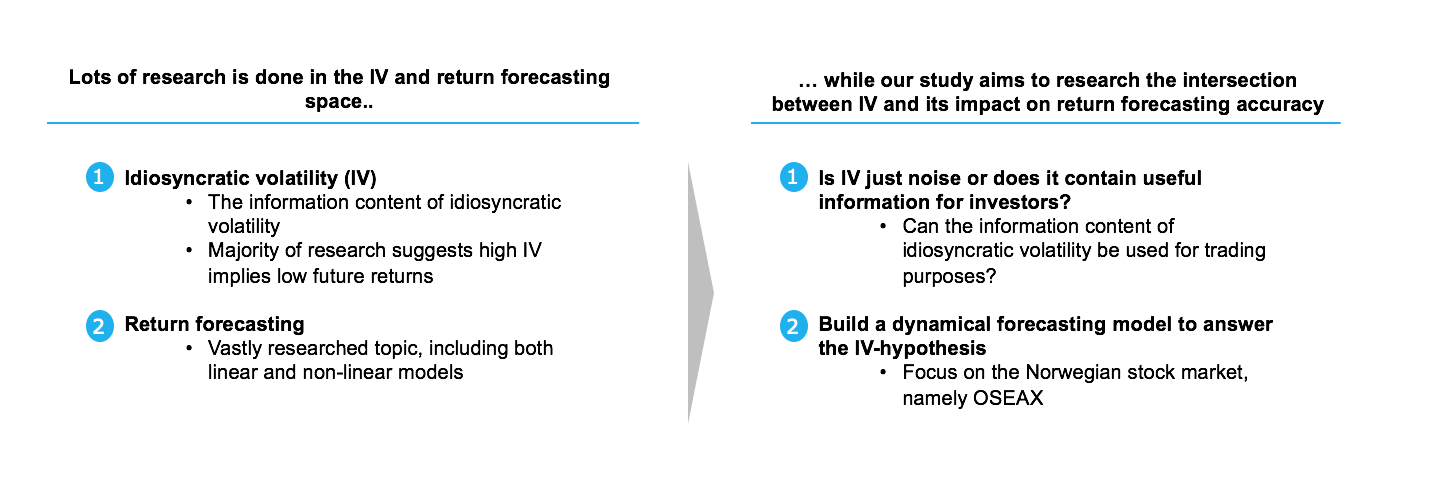
\includegraphics[scale = 0.5]{Plot/DummyLITREW.png}
    \caption{Regression: average daily IV percentage on annualized economic standard deviation}
    \label{IVtoVol}
\end{figure}

In this chapter we will review the literature in three sections. The two first sections will review what can be perceived as independent literature, while the third section will try to connect the first two sections and link them to the Norwegian stock market. 

\section*{Idiosyncratic volatility}

The behavior of stock returns, mainly in older and more consolidated stock markets such as those in the USA, has been studied for a long time.

The well-known Capital Asset Pricing Model (CAPM) proposed by Sharpe (1964) and Lintner (1965), is widely used to determine an asset's theoretical returns. Modern finance affirms that investors hold diversified stock portfolios to reduce idiosyncratic risk, which is a stock's specific risk. According to the CAPM, all investors should have a balanced market portfolio to eliminate all of the stock market's idiosyncratic risk. However, in practice, neither individual nor institutional investors hold such diversified portfolios and thus, some idiosyncratic risk is priced into their portfolios (Fu, 2009).

Various studies have attempted to complement the CAPM or to question its validity.Banz (1981) was an important work that analyzed the relation between returns and firms' market values. The author discovered the so-called size effect in stocks traded on the New York Stock Exchange, in which the performance of the stocks of smaller firms is superior to that of larger firms. According to Banz (1981), the size effect represents a failure of the CAPM specification because, for a specific beta, the average return of a stock with a lower market value is superior to that of a stock with a higher market value.

In addition, Banz (1981) served as the basis for other important and fundamental studies: Fama and French (1992), followed by Fama and French (1993), which developed their Three-Factor Model. Fama and French (1993) investigated the main risk factors associated with stock returns. Their model uses the following factors: market returns; the returns of a small minus big (SMB) variable, calculated as the average returns of small firm stock portfolios minus the average returns of large firm stock portfolios; and a high minus low (HML) variable, calculated as the difference in the returns of portfolios formed by firms with high and low book-to-market ratios. Fama and French (1993) conclude that the Three-Factor Model is superior to the CAPM in explaining average returns and that the model's three coefficients are simultaneously significant.

Various theories assume that idiosyncratic risk is positively correlated with stocks' expected returns. The idea behind this assumption is that investors who do not diversify their investments demand an additional return in order to bear the risk of their portfolios. The main exponents of these theories are Levy (1978), Merton (1973), and Malkiel and Xu (2002).

The empirical existence of a relationship between idiosyncratic risk and expected returns has been tested for a considerable amount of time. However, as highlighted in Fu and Schutte (2010), articles that find a positive relationship between these variables are almost equal in number to those that find no relation, or even a negative one. For example, Goyal and Santa-Clara (2003), who found evidence that market variance does not predict returns, should be highlighted. However, they found a positive and significant relationship between average stock variance, whose greatest component is idiosyncratic risk, and market returns. Goyal and Santa-Clara (2003) used a portfolio of stocks traded on the New York Stock Exchange (NYSE), American Stock Exchange (AMEX) and Nasdaq exchanges between August 1963 and December 1999.

Malkiel and Xu (2002) also found a positive relationship between idiosyncratic volatility and the cross-section of expected returns using the tests developed in Fama and Macbeth (1973) and Fama and French (1992). Malkiel and Xu (2002) arrived at the conclusion that idiosyncratic risk is more important than firm size, or beta, in explaining the cross-section of returns. Factors such as firm size, book-to-market ratio and liquidity were used as control variables in the cross-section regressions. The data covered stocks traded on the NYSE, AMEX and Nasdaq exchanges, as well as stocks traded on the Tokyo Stock Exchange (TSE), during the period from 1975 to 2000.

Kotiaho (2010) performed a similar study using stocks traded on the NYSE, AMEX and Nasdaq exchanges during the period from 1971 to 2008 and found a positive relation between stocks' idiosyncratic risks and expected returns, which was mainly due to the behavior of small-company stocks.

In contrast, other authors found no relation, or \textbf{even a negative one, between stocks' specific risk components and expected returns.}

Ang, Hodrick, Xing, and Zhang (2009) used data from 23 countries and concluded that high idiosyncratic volatility stocks generate lower future returns than low idiosyncratic volatility stocks. A previous article (Ang, Hodrick, Xing, & Zhang, 2006) showed a negative relation between a stock's monthly returns and its 1-month lagged idiosyncratic risk.

However, these conclusions are contested in Fu (2009), who contends that Ang et al.'s (2009) result was influenced by the stocks of smaller high idiosyncratic volatility firms. Fu (2009) replicated the method used in Ang et al. (2006) to estimate idiosyncratic volatility. The statistics of the series show, however, that idiosyncratic risk varies over time and its 1-month lagged value is therefore not a good proxy for the current month's expected risk. Thus, Fu (2009) proposes the use of the EGARCH model to estimate expected idiosyncratic volatility and this variable is included in the cross-section regressions along with other explanatory variables. The data covered the period from July 1963 to December 2006 for stocks traded on the NYSE, AMEX and Nasdaq exchanges. The results show a positive and statistically significant relation.

Bali and Cakici (2006) found no relation between an \textbf{equally weighted} stock portfolio's returns and its idiosyncratic risk Huang, Liu, Rhee, and Zhang (2010) contest these, as well as Ang et al.'s (2006) results. Huang et al.'s (2010) analysis shows that, in both cases, the obtained relation can be explained by short-term mean-reversion.

Angelidis (2010) investigates volatility's idiosyncratic component in 24 emerging countries. The study confirms the idea that the percentage of volatility that can be attributed to an asset's specific risk is lower in emerging markets than in developed markets, given the latter's greater efficiency. Angelidis (2010) also tested the relation between idiosyncratic risk and returns in these countries and the results show that idiosyncratic risk is a predictor of returns only when considered along with market risk.

In the case of the Norwegian market, some studies have already analyzed idiosyncratic risk.

\section*{Forecasting models}


\section*{Relationship between idiosyncratic volatility and return forecasting performance in the Norwegian stock market}

In relation to studies that focus on the Norwegian stock market